\label{section:vertex-area-chapter}
This section shows alternative methods to extend the idea of flat shading from triangles to vertices. The idea of flat shading is to draw all the pixels of a triangle with the same color. The extension of this approach is to split the surface of the triangle mesh likewise into regions around vertices and draw all pixels in these regions with the same color (Fig. \ref{fig:max-diagram-vertex-area}). Thus visualizing data given at the vertices of the mesh in a piecewise constant, not necessarily continuous way, which resembles the classical triangle flat shading. The aforementioned regions can easily be defined using barycentric coordinates and a simple GPU fragment program (Fig. \ref{fig:max-diagram-vertex-area}) can be used for each pixel to find out to which region it belongs and which color it should be painted with. Another interesting alternative data visualization technique given by the Gaussian curvature is presented at the end of this section.

%%%%%%%%%%%%%


\begin{figure}[!h]
    \centering
    \minipage[b]{.5\linewidth}
    \centering
    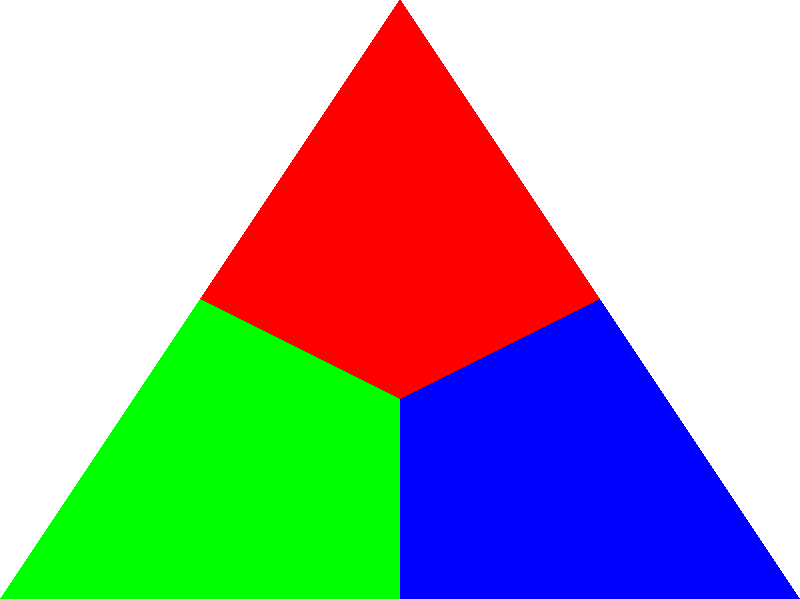
\includegraphics[scale=0.13]{images/max.png}
    \endminipage\hfill
    \minipage[b]{.5\linewidth}
    \centering
    \scalebox{0.45}{\begin{tikzpicture}
        \coordinate (J) at (3.8,3.6);
        \node[anchor=south west,inner sep=0] at (0,0) {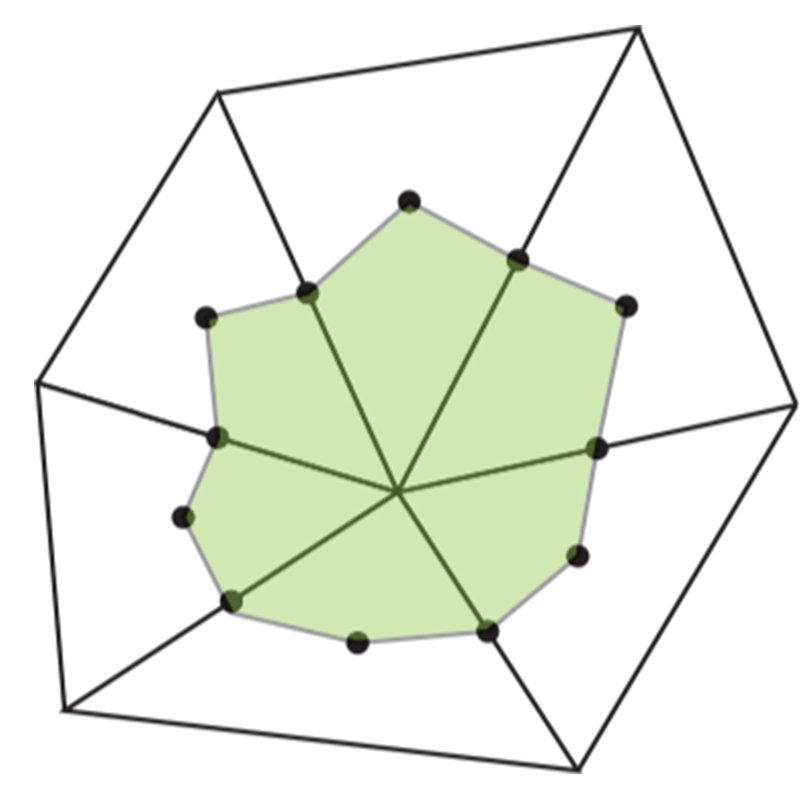
\includegraphics[scale=0.25]{images/vertex-area.png}};
        \draw (J) node [below left] {$j$};
        \filldraw (3.5,2.7) circle (2pt);
        \begin{scope}[line width=0.4mm, line cap=round]
            \draw (3.9,2.2) arc (295:360:0.7cm) node[near start,right] {$\theta_j$};
        \end{scope}
    \end{tikzpicture}}
    \endminipage
    \caption{On the left: Application of the max diagram algorithm on a triangle as illustrated in Section \ref{section:max-diagram}. On the right: region around a vertex; the angle defect is denoted with $\theta_j$.} \label{fig:max-diagram-vertex-area}
\end{figure}

%%%%%%%%%%%%%

\subsection{Max diagram - Vertex area} \label{section:max-diagram}
Passing barycentric coordinates to the \textit{fragment shader} will clearly demonstrate that we can get different results from the classic color interpolation \cite{WEBSITE:redbloggames}.
%----------
There are various approaches to color interpolation focusing on the distance from vertices. For each point in a triangle, we can easily determine its closest vertex, which we use as a cue for coloring.
Another approach, different from the above, can be defined as coloring vertex areas based on the maximum barycentric coordinate.
The color is given by the region closest to a vertex (Fig. \ref{fig:max-diagram-vertex-area}, Pseudocode \ref{appendix:max-diagram}).

%%%%%%%%%%%%%

\subsection{Vertex Flat Shading} \label{section:extend-flat-shading-lighting}
An extension of \textit{flat shading} would be to have each vertex area to be in one constant color (see Fig. \ref{figure:armadillo-efs}). This color can be taken using the normal at the vertex and the vertex position.
The color will then be computed as in \textit{Gouraud shading} avoiding the automatic interpolation of colors provided by OpenGL.
The idea is to compute the color per vertex but instead of linearly interpolating it in each triangle (as \textit{Gouraud shading} does) we color regions around a vertex with that constant color (using the GPU fragment program: max diagram \ref{section:max-diagram}).
To implement this approach, the barycentric coordinates, the vertex color, the normal at the vertex and the lighting calculations are passed to the \textit{fragment shader}.
In order to return the resulting color using the \textit{max diagram} algorithm, we have used a \textit{Geometry shader} that has access to all three vertex colors in the \textit{fragment shader}. (Pseudocodes: \ref{appendix:max-diagram}, \ref{appendix:vs-flat-shading-lighting}, \ref{appendix:geometry-shader})

\begin{figure}[!h]
    \centering
    \minipage[b]{.3\linewidth}
    \centering
    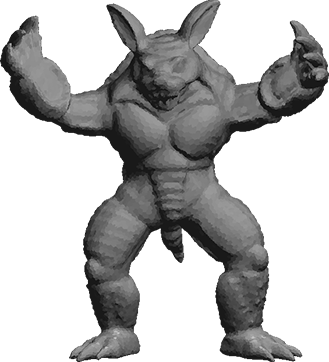
\includegraphics[scale=0.355]{images/armadillo-extendfs.png}
    \endminipage\hfill
    \minipage[b]{.3\linewidth}
    \centering
    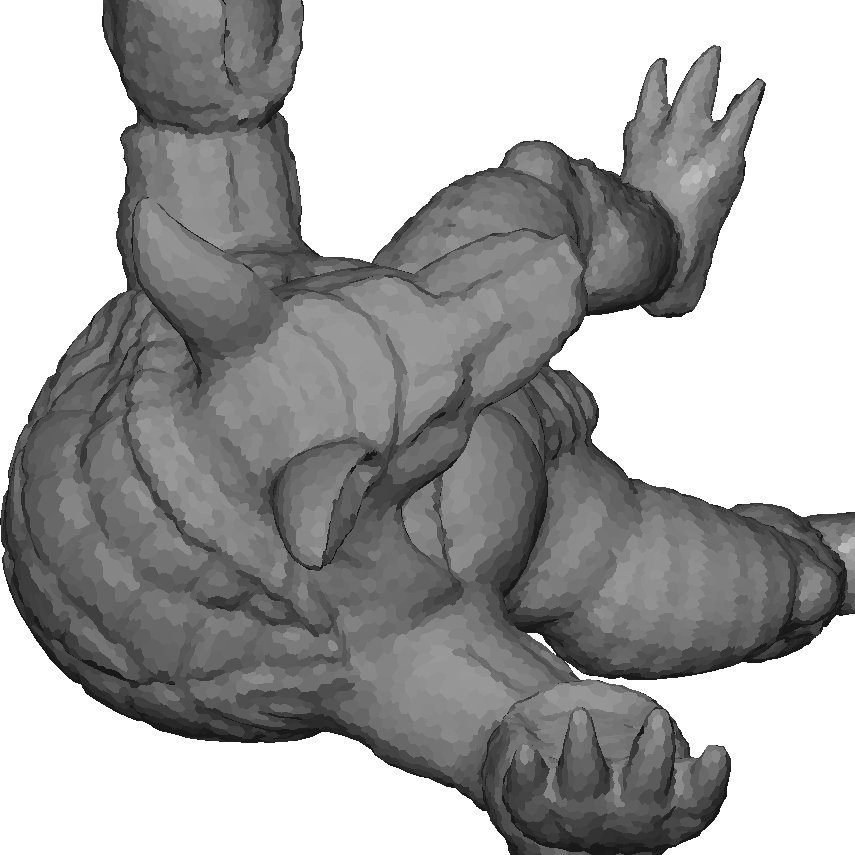
\includegraphics[scale=0.3]{images/armadillo-extendfs-1.png}
    \endminipage\hfill
    \minipage[b]{.3\linewidth}
    \centering
    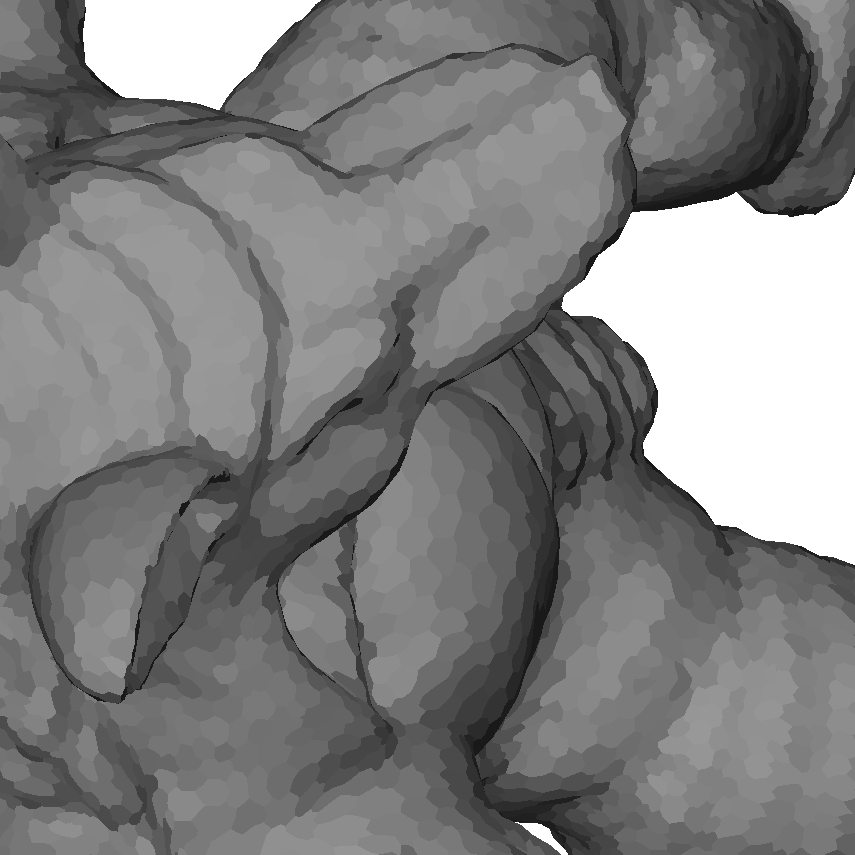
\includegraphics[scale=0.3]{images/armadillo-extendfs-2.png}
    \endminipage
    \caption{Vertex flat shading.}\label{figure:armadillo-efs}
\end{figure}


\subsection{Comparison between triangle flat shading, triangle Gouraud shading and vertex flat shading}
The standard approaches: \textit{triangle flat shading} and \textit{triangle Gouraud shading} are then compared with the new technique \textit{vertex flat shading}. In Fig. \ref{fig:comparison-icosahedron} we can see that the icosahedron where we have applied the vertex flat shading shader seems to be a good compromise since it preserves the original geometry and avoids creating triangle-like artifacts in the final result. Vertex regions look more realistic and less noisy than triangle regions. Moreover, Gouraud shading is prone to smoothing and losing many details in intricate and detailed meshes (see Fig. \ref{fig:comparison-fs-efs-gs}).
\begin{figure}[!h]
    \centering
    \minipage[b]{.3\linewidth}
    \centering
    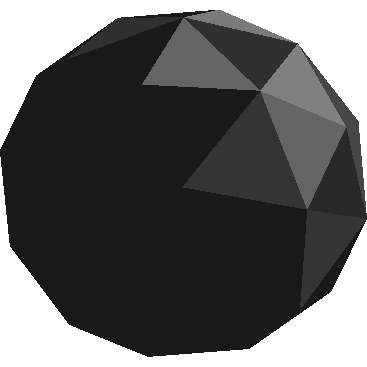
\includegraphics[scale=0.5]{images/flatshading.png}
    \label{fig:flat-shading-triangle}
    \endminipage\hfill
    \minipage[b]{.3\linewidth}
    \centering
    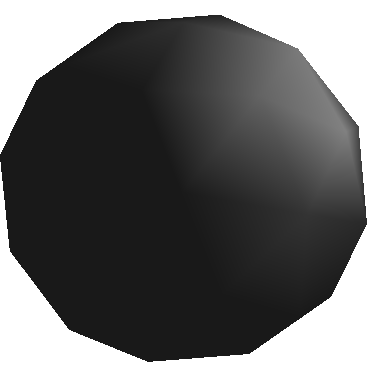
\includegraphics[scale=0.5]{images/gouraudshading.png}
    \label{fig:gouraud-shading}
    \endminipage\hfill
    \minipage[b]{.3\linewidth}
    \centering
    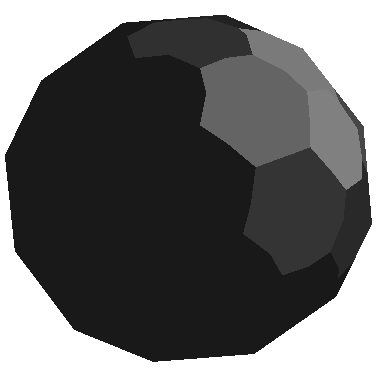
\includegraphics[scale=0.5]{images/extentflatshading.png}\label{fig:flat-shading-vertex}
    \endminipage
    \caption{Comparison between: triangle flat shading, triangle Gouraud shading and vertex flat shading.}
    \label{fig:comparison-icosahedron}
\end{figure}

\begin{figure}[!h]
    \centering
    \minipage[b]{.33\linewidth}
    \centering
    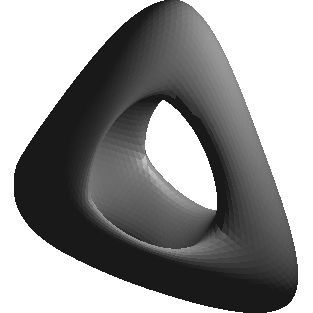
\includegraphics[scale=0.6]{images/genus-fs.png}
    \endminipage\hfill
    \centering
    \minipage[b]{.33\linewidth}
    \centering
    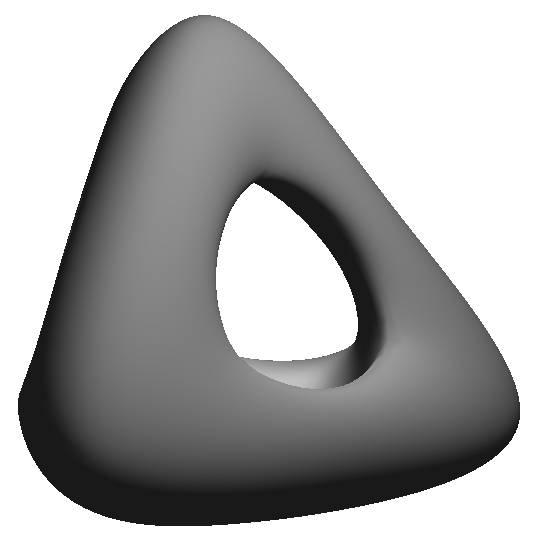
\includegraphics[scale=0.6]{images/genus-gs.png}
    \endminipage\hfill
    \minipage[b]{.33\linewidth}
    \centering
    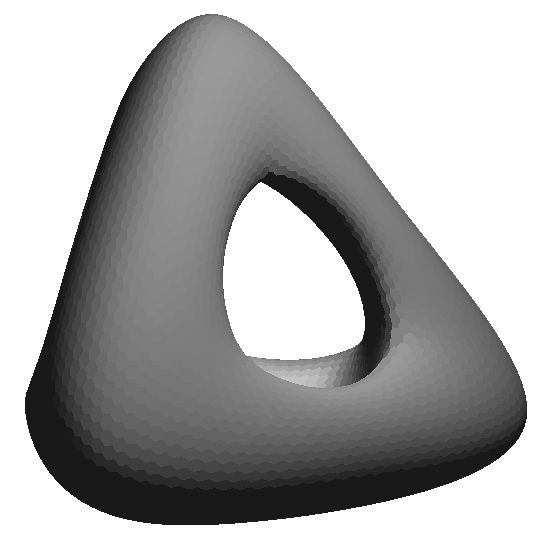
\includegraphics[scale=0.6]{images/genus-efs.png}
    \endminipage\hfill
    \minipage[b]{.33\linewidth}
    \centering
    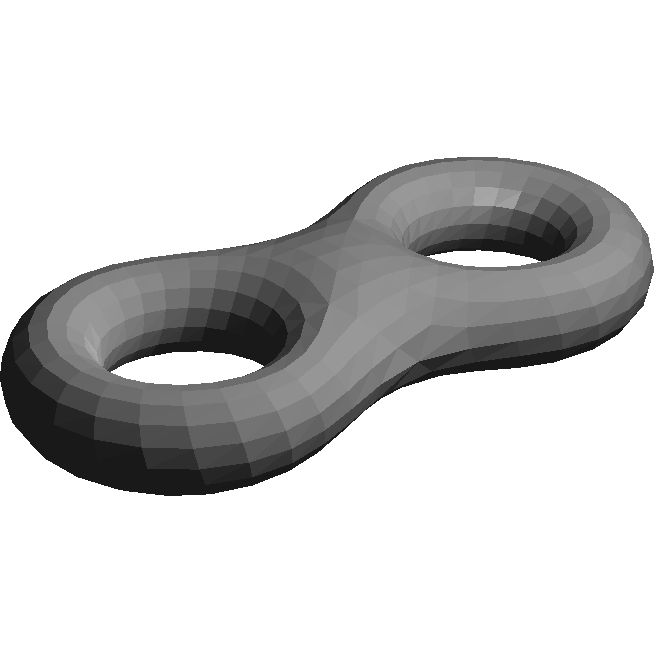
\includegraphics[scale=0.35]{images/eight-fs.png}
    \endminipage\hfill
    \centering
    \minipage[b]{.33\linewidth}
    \centering
    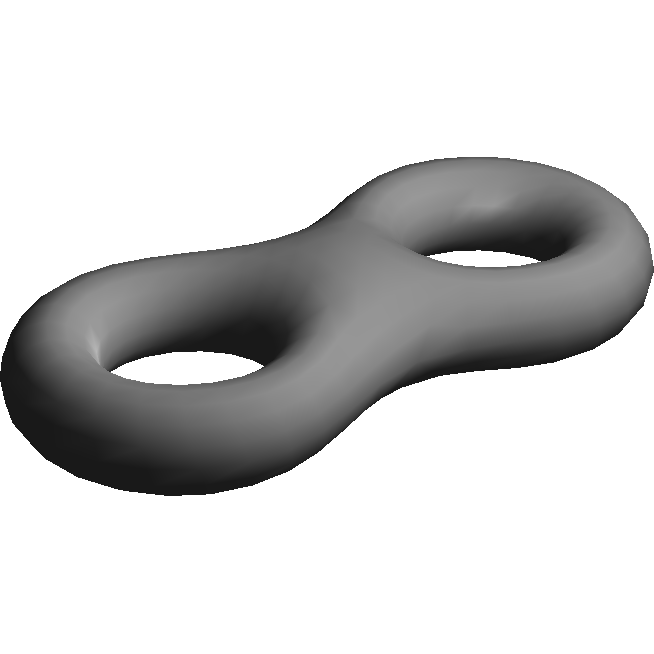
\includegraphics[scale=0.35]{images/eight-gs.png}
    \endminipage\hfill
    \minipage[b]{.33\linewidth}
    \centering
    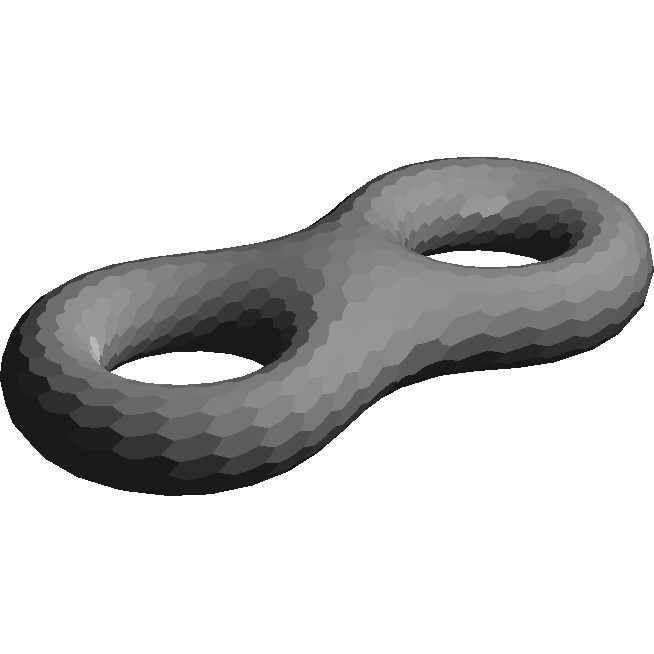
\includegraphics[scale=0.35]{images/eight-efs.png}
    \endminipage\hfill
    \centering
    \minipage[b]{.33\linewidth}
    \centering
    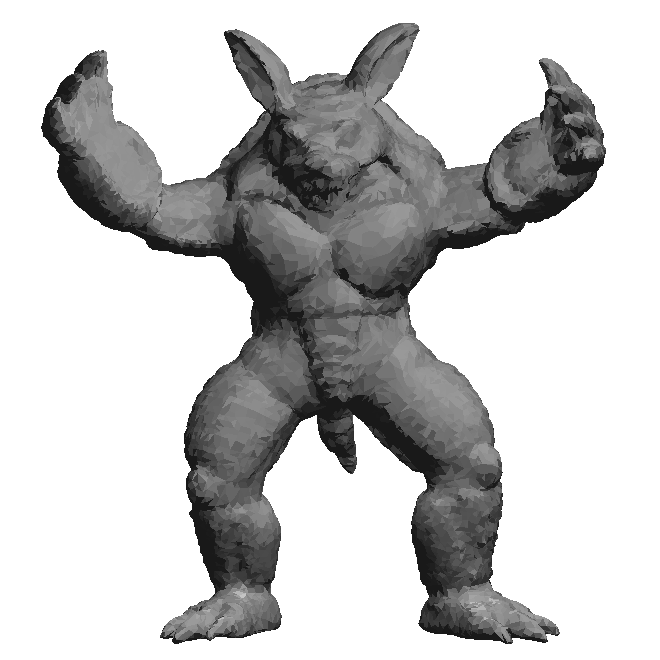
\includegraphics[scale=0.6]{images/armadillo-fs.png}
    \endminipage\hfill
    \centering
    \minipage[b]{.33\linewidth}
    \centering
    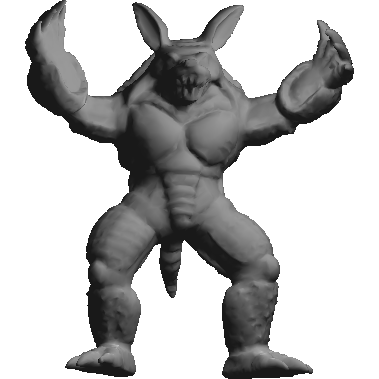
\includegraphics[scale=0.6]{images/armadillo-gs.png}
    \endminipage\hfill
    \minipage[b]{.33\linewidth}
    \centering
    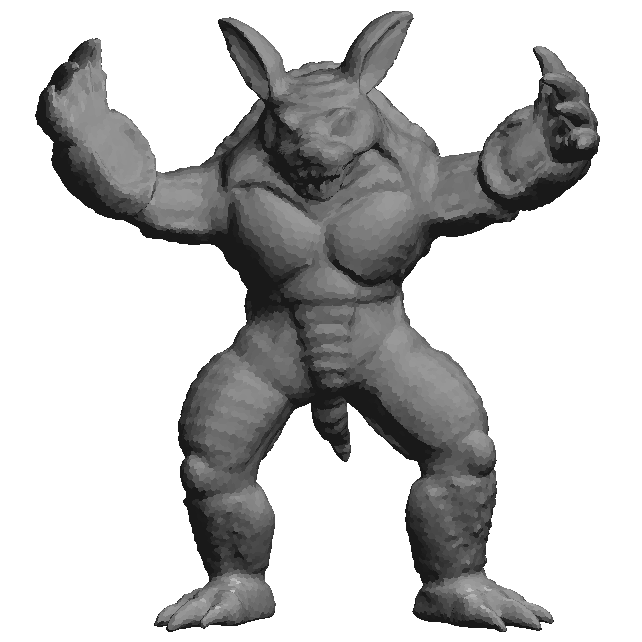
\includegraphics[scale=0.6]{images/armadillo-efs.png}
    \endminipage\hfill
    \minipage[b]{.33\linewidth}
    \centering
    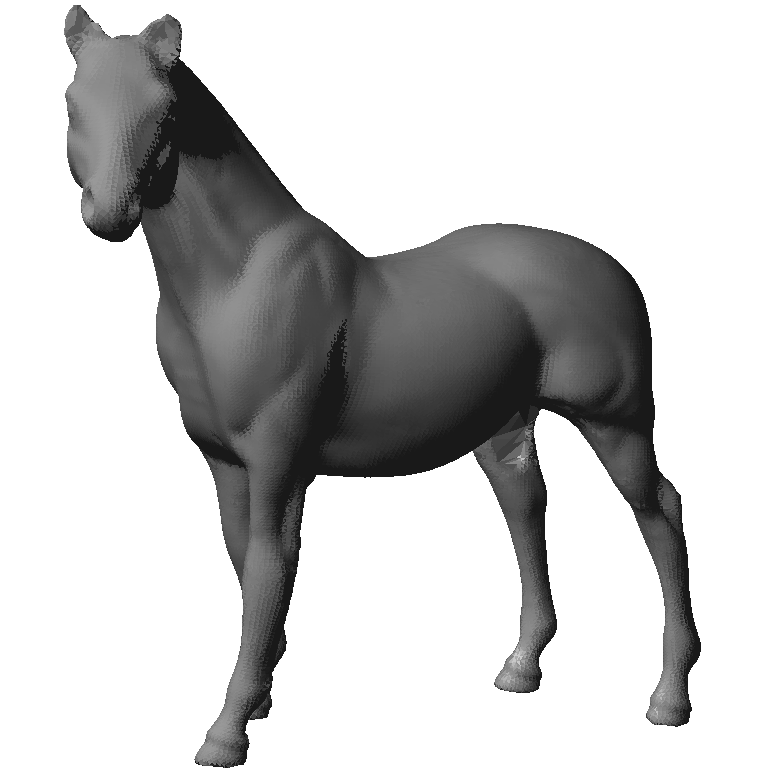
\includegraphics[scale=0.39]{images/horse-fs.png}
    \endminipage\hfill
    \centering
    \minipage[b]{.33\linewidth}
    \centering
    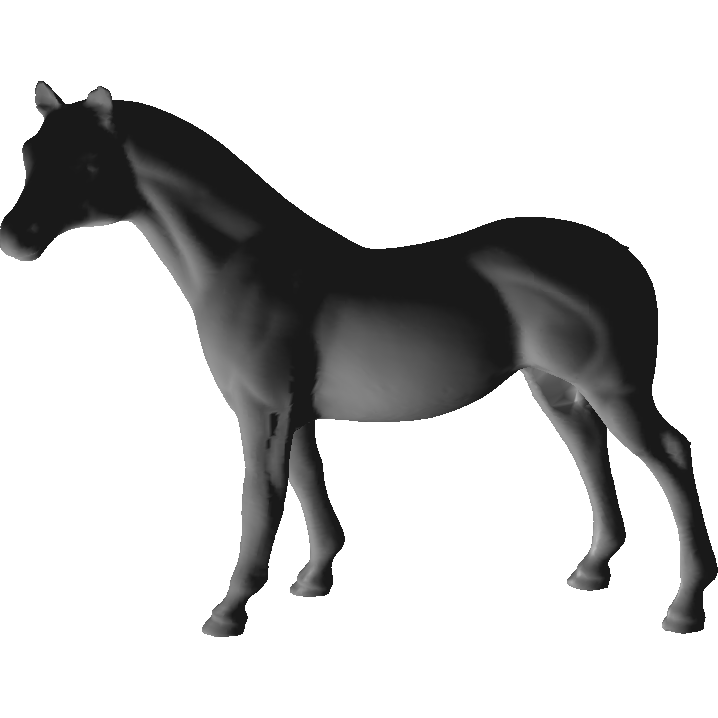
\includegraphics[scale=0.39]{images/horse-gs.png}
    \endminipage\hfill
    \minipage[b]{.33\linewidth}
    \centering
    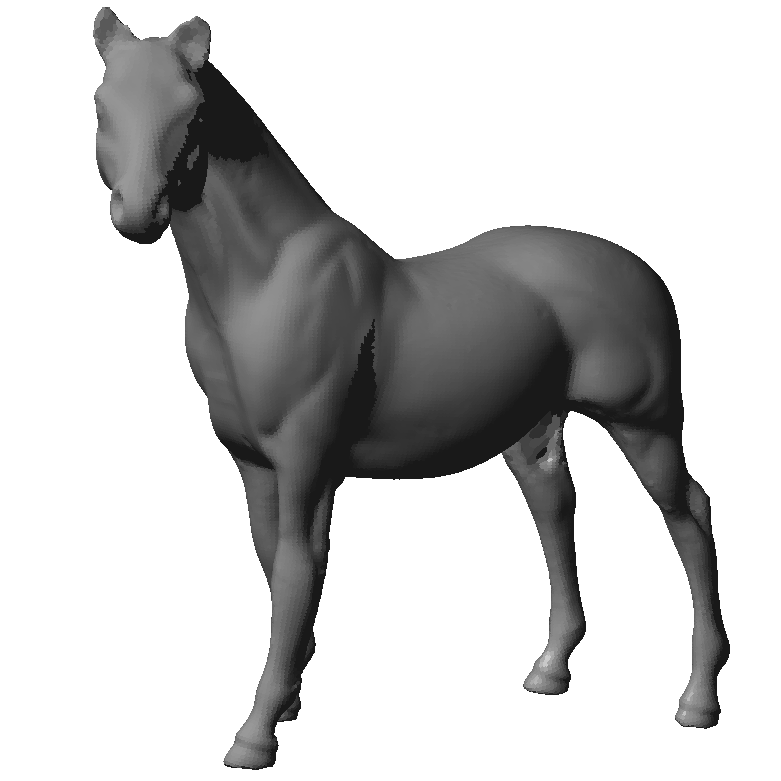
\includegraphics[scale=0.39]{images/horse-efs.png}
    \endminipage\hfill
    \caption{On the left: Triangle flat shading. On the center: Triangle Gouraud shading. On the right: Vertex flat shading.}
    \label{fig:comparison-fs-efs-gs}
\end{figure}

%%%
\subsection{Gaussian curvature}
\label{section:vertex-area-gaussian-curvature}
Another interesting alternative data visualization technique is given computing the \textit{Gaussian curvature} per vertex. That can be done by summing up, angles of the triangles adjacent to the vertex $V$ at $V$, and then subtracting this value from $2\pi$.
Having obtained this value, called \textit{angle defect} (Fig. \ref{fig:max-diagram-vertex-area}), we map it linearly to a color range.
The resulting color will be the vertex flat shading visualisation of \textit{Gaussian curvature} (See Section \ref{section:localaveraging} and \ref{section:gaussian-curvature-intro}).
$$K(V) = (2\pi - \sum_j \theta_j)/\mathcal{A}_{Mixed}$$

%%%%%%%%

\subsection{Constant Gaussian curvature}
\label{section:gc-curvature}
\textit{Constant Gaussian curvature} returns a constant color around each vertex using the max diagram algorithm (Fig. \ref{fig:max-diagram-vertex-area}, pseudocode \ref{appendix:vs-curvature}). The value $K(V)$ is mapped to a color range to get the corresponding curvature color (see Fig. \ref{fig:color-range-curvature}). This process is made separately for each vertex of the triangle and consequently, using the technique of max-diagram explained above (see section \ref{section:max-diagram}), the final resulting constant color is returned.
\begin{figure}[!h]
    \centering
    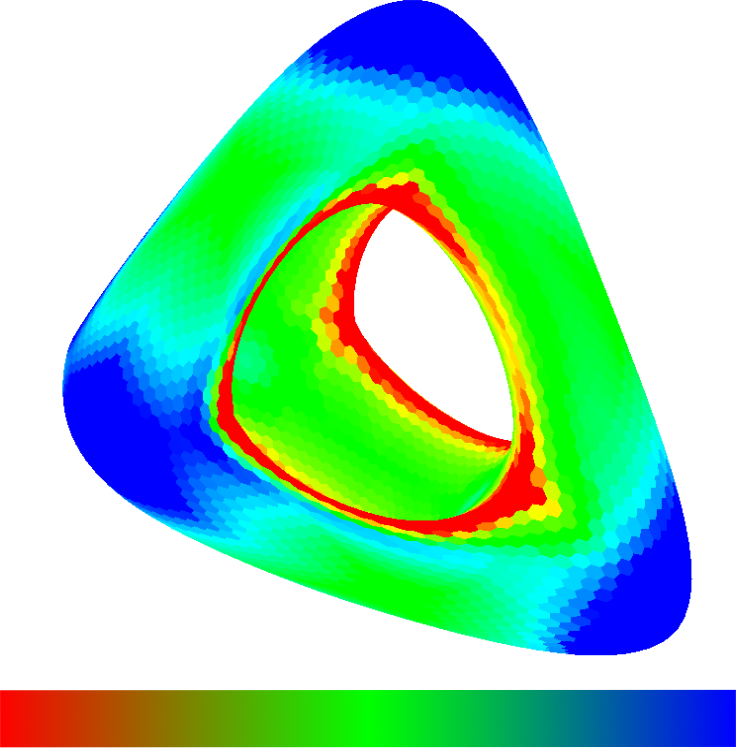
\includegraphics[width=6cm]{images/gradient-curvature.png}
    \caption{Color bar showing respective colors for negative, flat and positive curvatures. Negative curvatures are mapped to red, flat curvatures to green and positive curvatures to blue.} \label{fig:color-range-curvature}
\end{figure}


\begin{figure}[!h]
    \centering
    \minipage[b]{.5\linewidth}
    \centering
    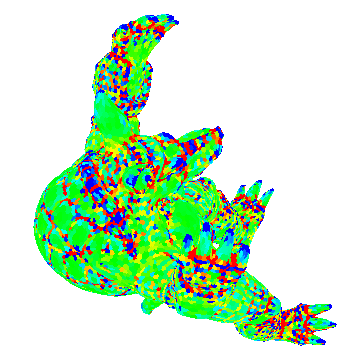
\includegraphics[scale=1.0]{images/gc-armadillo-top.png}
    \endminipage\hfill
    \minipage[b]{.5\linewidth}
    \centering
    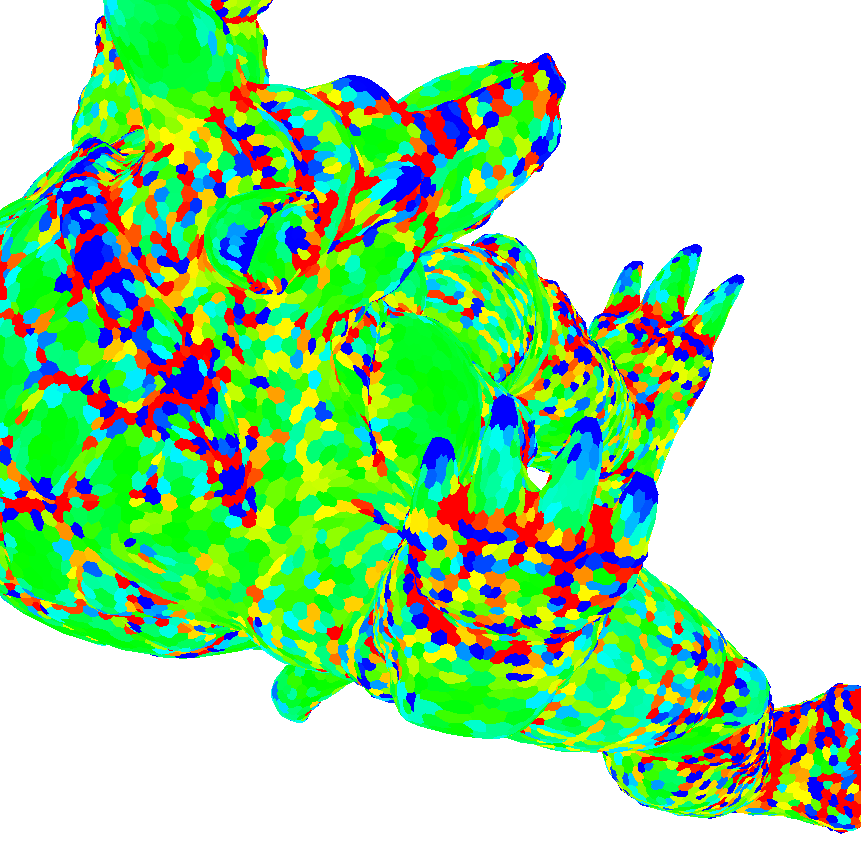
\includegraphics[scale=0.4]{images/gc-detail-armadillo-top.png}
    \endminipage
    \caption{Constant Gaussian curvature} \label{fig:gc-detail}
\end{figure}



\subsection{Gouraud Gaussian curvature}
\textit{Gouraud Gaussian curvature} computes the curvature per vertex, converts it to color, and linearly interpolates it. The idea is to calculate the \textit{Gaussian curvature} as explained above (mapping the color into a color range to get the corresponding color per vertex) but instead of returning the constant color using a max-diagram approach, we just return the interpolation of values obtained for each triangle.

\begin{figure}[!h]
    \centering
    \minipage[b]{.5\linewidth}
    \centering
    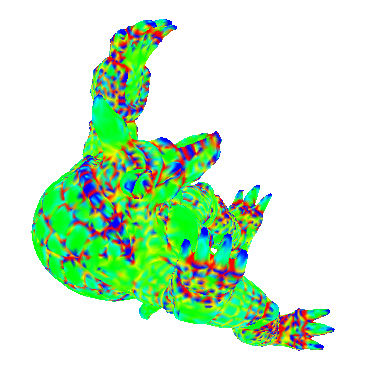
\includegraphics[scale=1.0]{images/gci-armadillo-top.png}
    \endminipage\hfill
    \minipage[b]{.5\linewidth}
    \centering
    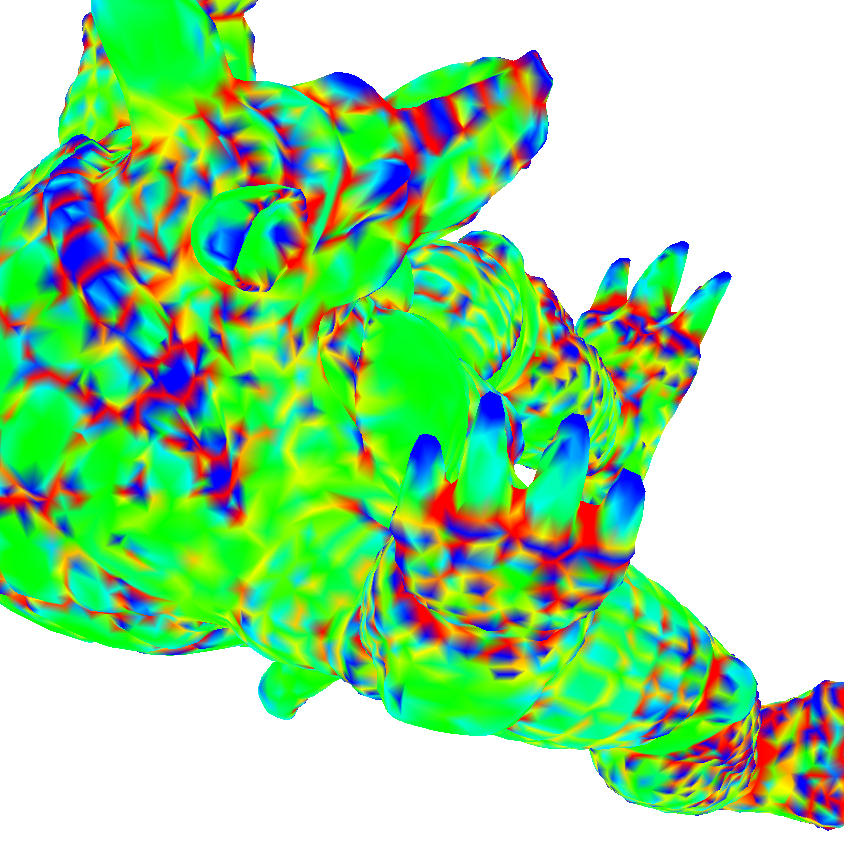
\includegraphics[scale=0.4]{images/gci-detail-armadillo-top.png}
    \endminipage
    \caption{Gouraud Gaussian curvature} \label{fig:gci-detail}
\end{figure}


\subsection{Evaluation and Comparison between constant Gaussian curvature per vertex and Gouraud Gaussian curvature}
In \textit{constant Gaussian curvature} (Fig. \ref{fig:gc-detail}) each vertex area is colored applying the \textit{max diagram} algorithm. Instead, in \textit{Gouraud Gaussian curvature} (Fig. \ref{fig:gci-detail}) the color is obtained with linear interpolation.
Visualization of the Gauss curvatures of the model as colors from blue (highest values of curvature) to red (lower values of curvature) highlighs the geometry of meshes in Fig. \ref{fig:comparison-gc-gci}.
These changes of curvature, positive (blue), flat (green) and negative regions (red), better emphasizes the 3-dimensionality of the model.
\textit{Gouraud Gaussian curvature} is smoother, which results in a loss of small details. This is particularly evident in armadillo's legs mesh. Instead, \textit{constant Gaussian curvature} generates sharper edges with piecewise-flat regions which slightly degrades the 3-dimensional perception of the model.
On the other hand, it preserves the details of the given geometry, which can be particularly useful for data visualization purposes.

\begin{figure}[!h]
    \centering
    \minipage[b]{.5\linewidth}
    \centering
    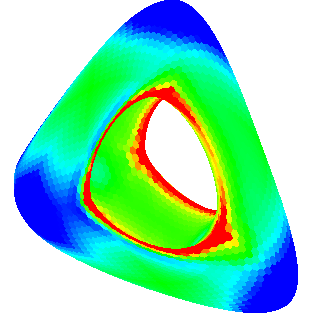
\includegraphics[scale=0.7]{images/gc-genus.png}
    \endminipage\hfill
    \minipage[b]{.5\linewidth}
    \centering
    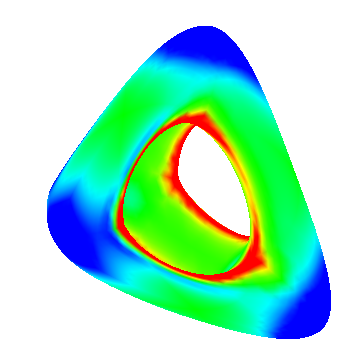
\includegraphics[scale=0.7]{images/gci-genus.png}
    \endminipage\hfill
    \minipage[b]{.5\linewidth}
    \centering
    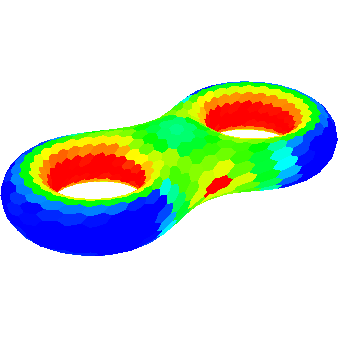
\includegraphics[scale=0.75]{images/gc-eight.png}
    \endminipage\hfill
    \minipage[b]{.5\linewidth}
    \centering
    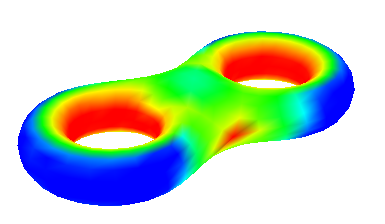
\includegraphics[scale=0.75]{images/gci-eight.png}
    \endminipage\hfill
    \minipage[b]{.5\linewidth}
    \centering
    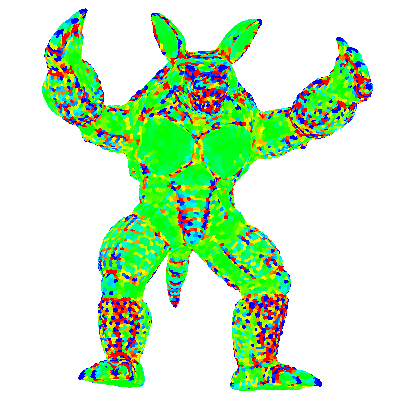
\includegraphics[scale=0.75]{images/gc-armadillo.png}
    \endminipage\hfill
    \minipage[b]{.5\linewidth}
    \centering
    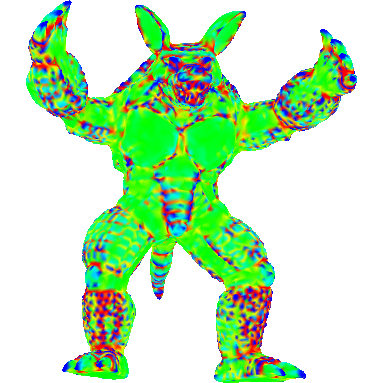
\includegraphics[scale=0.75]{images/gci-armadillo.png}
    \endminipage\hfill
    \minipage[b]{.5\linewidth}
    \centering
    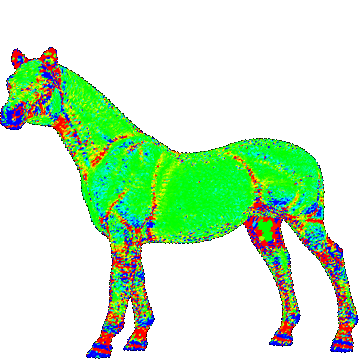
\includegraphics[scale=0.75]{images/gc-horse.png}
    \endminipage\hfill
    \minipage[b]{.5\linewidth}
    \centering
    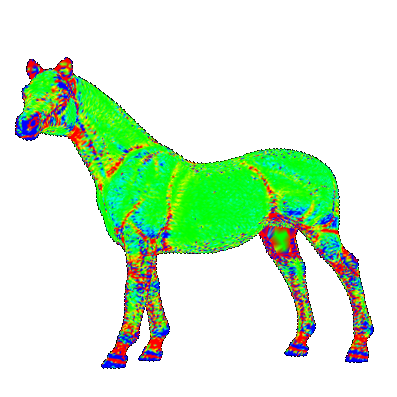
\includegraphics[scale=0.75]{images/gci-horse.png}
    \endminipage
    \caption{On the left: Constant Gaussian curvature. On the right: Gouraud Gaussian curvature.}
    \label{fig:comparison-gc-gci}
\end{figure}

